\chapter{Key Infrastructure}
This chapter will present the concept of \gls{IBE} and \gls{IBS}, and why it is highly applicable to use this type of cryptography in \gls{NDN}. 
Then the possibilities to use the file synchronization module to do key distribution and revocation will be introduced.

\section{Identity-Based Cryptography}\label{ibc}
\gls{IBE} was first proposed by Shamir~\cite{DBLP:conf/crypto/Shamir84} in 1984. 
The concept of \gls{IBE} builds upon every user having an \gls{ID} that is used as the public key. 
This \gls{ID} can be anything, i.e. email, phone number, \gls{SSN}, or a Name (~\autoref{name}).
This eliminates the need of certificates.
Shamir did propose a scheme for \gls{IBS}, but not a scheme for \gls{IBE}. 
The \gls{IBE} implementation remained unsolved until 2001, when Dan Boneh and Matthew K. Franklin proposed~\cite{DBLP:conf/crypto/BonehF01}.
However the scheme has only been shown to be secure with a random oracles model~\cite{DBLP:journals/iacr/Waters04}, hence less practical.


\gls{IBE} is based upon performing cryptography with a publicly know \gls{ID}.
Since the \gls{ID} can be practically anything it is highly applicable for \gls{NDN} where the \gls{ID} can be a Name (``/ndn/no/ntnu/haakon'').
Hence the Name becomes the public key. 

There is a \gls{TTP} in \gls{IBE} that is called \gls{PKG}.
The \gls{PKG}s task is to produce a secret key that corresponds to a given ID and provide 

\begin{enumerate}\label{ibc-methods}
  \item \texttt{Setup()} generates a key pair, \gls{MPK} and \gls{MSK}. These keys are used by only the \gls{PKG} to extracting secret keys, encryption and decryption.
  \item \texttt{Extract(MPK\textsubscript{PKG}, MSK\textsubscript{PKG}, ID\textsubscript{device})} generates a secret key from a given ID. 
  \item \texttt{Encrypt(MPK\textsubscript{PKG}, ID\textsubscript{device}, message)} encrypts the message.
  \item \texttt{Decrypt(MPK\textsubscript{PKG}, SK\textsubscript{device}, cipher)} decrypts the cipher generated from the encryption.
  \item \texttt{Signing(MPK\textsubscript{PKG}, SK\textsubscript{device}, message)} signs a hash digest of the message (e.g. \gls{SHA1}).
  \item \texttt{Verify(MPK\textsubscript{PKG}, ID\textsubscript{device}, message, signature)} verifies the signature.
\end{enumerate}

\begin{figure}[ht]
  \centering
  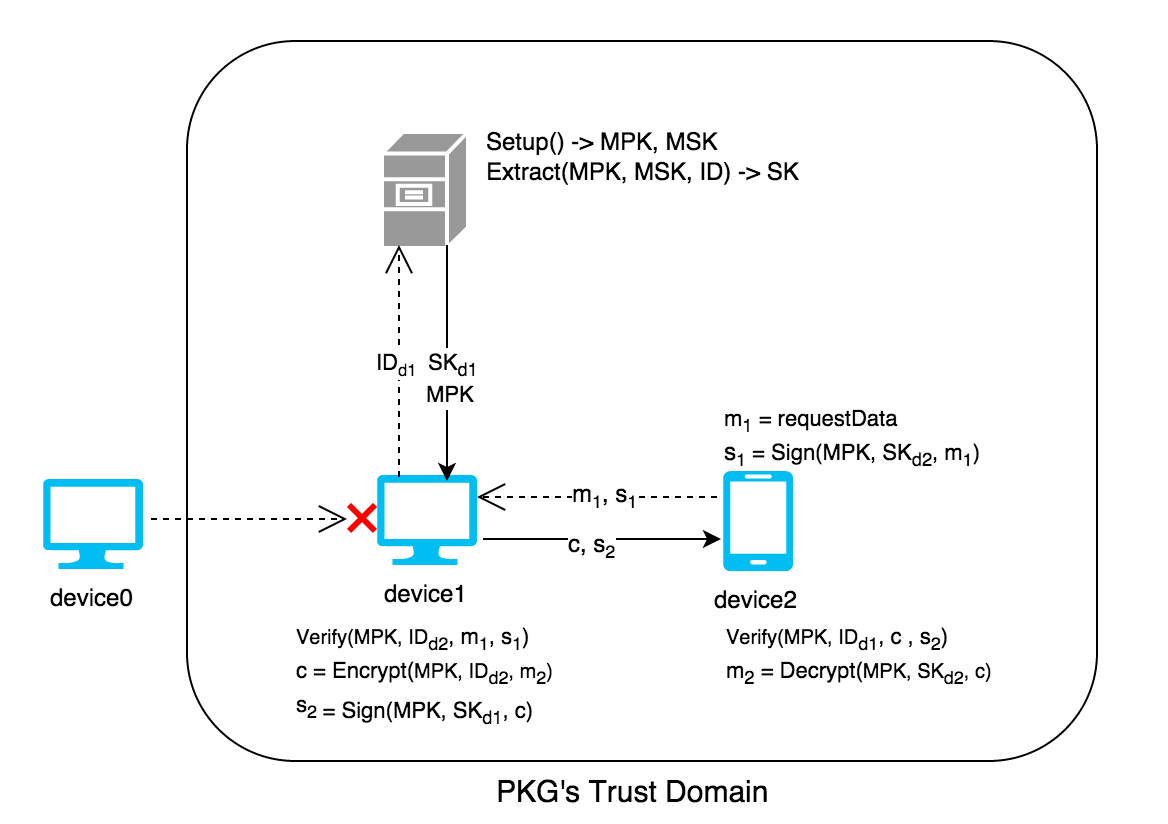
\includegraphics[width=1\textwidth]{pkg_functions.png}
  \caption{Methods of an IBC systems illustrated in action.}
  \label{fig:pkg_functions}
\end{figure}

To encrypt a message with \gls{IBE}, the user encrypts a \gls{CEK} with the recipients \gls{ID}.
The user encrypts the message using the \gls{CEK} together with symmetric encryption~\cite[section 2.2.2]{rfc5408}, and sends both the encrypted \gls{CEK} and the encrypted content to the requester. 

Some drawbacks related to \gls{IBE} are listed below:
\begin{enumerate}
	\item If \gls{PKG} is compromised. Adversary has secret key to all nodes that used the compromised \gls{PKG}
	\item \gls{PKG} can read and write messages related to the node, because it has all secret keys, i.e. \gls{MITM}.
	\item \gls{PKG} and the requesting node has to establish a secure channel. 
\end{enumerate}

\section{Identity-Based Cryptography - Secureness}

A random oracle is like a ``black box'' that outputs truly random numbers.
When designing protocols in cryptography one first usually designs an ideal system where all parties have random oracle access, then proves the security.
Second, one replaces the oracle access with a hash function.
This gives an implementation of an ideal system in the real world, but without random oracles~\cite{DBLP:conf/ccs/BellareR93}. 
It is just fine to make statements based on the ideal system, but debatable whether the same statements yields for the implementation in the real world.
Canetti et al. concluded that there exist secure schemes in the \textit{Random Oracle Model}, but for which any implementation of the random oracle results in insecure schemes~\cite{DBLP:journals/jacm/CanettiGH04}.
Boneh and Franklins \gls{IBE} scheme is only secure when using random oracles.

Following the \textit{Standard Model} one does not resort to the random oracle heuristic and does not rely on non-standard complexity assumptions.
Hence proving security in the standard model is preferably.
In 2014 Boneh and Boyen proposed a fully secure scheme in the standard model~\cite{DBLP:conf/crypto/BonehB04}.
However it is not efficient. 

First practical scheme was ~\cite{DBLP:journals/iacr/Waters04}.
But as David Naccache states in his paper~\cite{DBLP:journals/iacr/Naccache05}, Waters' scheme without random oracles introduces too large public parameters (164\gls{KB}!).
Naccache proves that he was able to construct a practical and fully secure scheme in the standard model based on the \gls{DBDH} assumption.
The scheme is a modification of Waters' scheme, but with public parameters of just a few \gls{KB} size.

Brent Waters created a fully secure \gls{IBE} system with short parameters under simple assumption in 2009~\cite{DBLP:conf/crypto/Waters09}.

To understand the mathematical assumptions for \gls{IBE}, the reader should take a look at~\cite[section 3]{DBLP:conf/crypto/BonehF01} for details about bilinear maps and~\gls{BDH}.

\section{Key Distribution}
Instead of in \gls{PKI} where each public key is signed by a certificate authority and the generated certificate is sent as a response in \gls{HTTPS} then validated by the the client, I want to make the certificate authority obsolete by distributing every \gls{ID} (public key) issued by the \gls{PKG}.
This can be done through an IDSync application built upon the application presented in~\autoref{file-sync}.
In~\autoref{fig:pkg_sync} we see that the \gls{PKG} multicasts the \gls{ID} list to all devices that have joined the domain.
Each device can verify the integrity and authenticity of the sync state Data and be sure that the \gls{ID} list surely originates from its own \gls{PKG}.
\begin{figure}[ht]
  \centering
  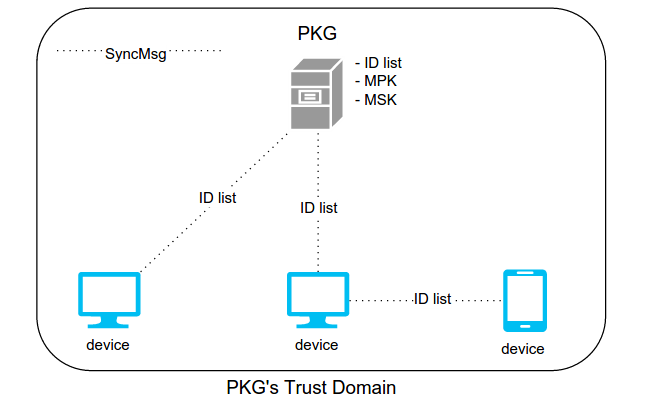
\includegraphics[width=1\textwidth]{pkg_sync.png}
  \caption{IDSync with tree devices and a PKG.}
  \label{fig:pkg_sync}
\end{figure}

\section{Key Revocation}
Few alternatives to revocation scheme in \gls{IBE}.
Key Revocation in IBE ~\cite{DBLP:journals/iacr/BoldyrevaGK12} 
One suggestion is to allocate secret keys with the public key combined with some sort of date, e.g. month-year or just year. 
In this alternative a user has to renew its secret key each time the date changes, i.e. either the month or the year depending on the date format.
The problem with the revocation solution is that it is cumbersome for the \gls{PKG}.


Key revocation becomes obsolete with the IDSync distribution solution. 
